%%
%% This is file `sample-sigconf.tex',
%% generated with the docstrip utility.
%%
%% The original source files were:
%%
%% samples.dtx  (with options: `sigconf')
%% 
%% IMPORTANT NOTICE:
%% 
%% For the copyright see the source file.
%% 
%% Any modified versions of this file must be renamed
%% with new filenames distinct from sample-sigconf.tex.
%% 
%% For distribution of the original source see the terms
%% for copying and modification in the file samples.dtx.
%% 
%% This generated file may be distributed as long as the
%% original source files, as listed above, are part of the
%% same distribution. (The sources need not necessarily be
%% in the same archive or directory.)
%%
%% Commands for TeXCount
%TC:macro \cite [option:text,text]
%TC:macro \citep [option:text,text]
%TC:macro \citet [option:text,text]
%TC:envir table 0 1
%TC:envir table* 0 1
%TC:envir tabular [ignore] word
%TC:envir displaymath 0 word
%TC:envir math 0 word
%TC:envir comment 0 0
%%


%%
%% The first command in your LaTeX source must be the \documentclass command.
\documentclass[sigconf]{acmart}

 

%% NOTE that a single column version may be required for 
%% submission and peer review. This can be done by changing
%% the \documentclass[...]{acmart} in this template to 
%% \documentclass[manuscript,screen]{acmart}
%% 
%% To ensure 100% compatibility, please check the white list of
%% approved LaTeX packages to be used with the Master Article Template at
%% https://www.acm.org/publications/taps/whitelist-of-latex-packages 
%% before creating your document. The white list page provides 
%% information on how to submit additional LaTeX packages for 
%% review and adoption.
%% Fonts used in the template cannot be substituted; margin 
%% adjustments are not allowed.
%%
%%
%% \BibTeX command to typeset BibTeX logo in the docs
\AtBeginDocument{%
  \providecommand\BibTeX{{%
    \normalfont B\kern-0.5em{\scshape i\kern-0.25em b}\kern-0.8em\TeX}}}

%% Rights management information.  This information is sent to you
%% when you complete the rights form.  These commands have SAMPLE
%% values in them; it is your responsibility as an author to replace
%% the commands and values with those provided to you when you
%% complete the rights form.
\copyrightyear{2025} 
\acmYear{2025} 
\setcopyright{acmlicensed}\acmConference[ICAIF '25]{6th ACM International Conference on AI in Finance}{November 15--18, 2025}{Singapore}
\acmBooktitle{6th ACM International Conference on AI in Finance (ICAIF '25), November 15--18, 2025, Singapore}
\acmPrice{15.00}
\acmDOI{10.1145/3604237.3626838}
\acmISBN{979-8-4007-0240-2/23/11}




%%
%% Submission ID.
%% Use this when submitting an article to a sponsored event. You'll
%% receive a unique submission ID from the organizers
%% of the event, and this ID should be used as the parameter to this command.
%%\acmSubmissionID{123-A56-BU3}

%%
%% For managing citations, it is recommended to use bibliography
%% files in BibTeX format.
%%
%% You can then either use BibTeX with the ACM-Reference-Format style,
%% or BibLaTeX with the acmnumeric or acmauthoryear sytles, that include
%% support for advanced citation of software artefact from the
%% biblatex-software package, also separately available on CTAN.
%%
%% Look at the sample-*-biblatex.tex files for templates showcasing
%% the biblatex styles.
%%

%%
%% The majority of ACM publications use numbered citations and
%% references.  The command \citestyle{authoryear} switches to the
%% "author year" style.
%%
%% If you are preparing content for an event
%% sponsored by ACM SIGGRAPH, you must use the "author year" style of
%% citations and references.
%% Uncommenting
%% the next command will enable that style.
%%\citestyle{acmauthoryear}

%%
%% end of the preamble, start of the body of the document source.


%% Bibliography style
% \RequirePackage[
%   datamodel=acmdatamodel,
%   style=acmnumeric,
%   ]{biblatex}


%% Declare bibliography sources (one \addbibresource command per source)
% \addbibresource{references.bib} 
% \usepackage{natbib}
% \bibliographystyle{unsrtnat}
\bibliographystyle{ACM-Reference-Format}



\begin{document}

%%
%% The "title" command has an optional parameter,
%% allowing the author to define a "short title" to be used in page headers.
\title{In-Context Learning for Smarter Fraud Detection in Remote Secondhand Transactions}

%%
%% The "author" command and its associated commands are used to define
%% the authors and their affiliations.
%% Of note is the shared affiliation of the first two authors, and the
%% "authornote" and "authornotemark" commands
%% used to denote shared contribution to the research.


\author{Hyunwoo Kim}
\orcid{xxxxxxxx}
% \authornote{These authors contributed equally to this research}
\affiliation{%
  \institution{Danggeun Pay Inc.}
  \state{Seoul}
  \country{Republic of Korea}
}
\email{peter.kim@daangnpay.com}



\author{Hyunmyoung Oh}
\orcid{xxxxxxxx}
% \authornotemark[1]
\affiliation{%
  \institution{Danggeun Pay Inc.}
  \state{Seoul}
  \country{Republic of Korea}
}
\email{hammer@daangnpay.com}



\author{Sunghyon Kyeong}
\orcid{0000-0002-9095-5219}
\authornote{Corresponding author}
\affiliation{%
  \institution{Danggeun Pay Inc.}
  \state{Seoul}
  \country{Republic of Korea}
}
\email{devyn@daangnpay.com}




%%
%% By default, the full list of authors will be used in the page
%% headers. Often, this list is too long, and will overlap
%% other information printed in the page headers. This command allows
%% the author to define a more concise list
%% of authors' names for this purpose.
\renewcommand{\shortauthors}{Kim et al.}

%%
%% The abstract is a short summary of the work to be presented in the
%% article.
\begin{abstract}
this part is not ready yet.
\end{abstract}

%%
%% The code below is generated by the tool at http://dl.acm.org/ccs.cfm.
%% Please copy and paste the code instead of the example below.
%%
\begin{CCSXML}
  <ccs2012>
    <concept>
      <concept_id>10010147.10010178.10010179</concept_id>
      <concept_desc>Computing methodologies~Natural language processing</concept_desc>
      <concept_significance>500</concept_significance>
    </concept>
    <concept>
      <concept_id>10010147.10010257</concept_id>
      <concept_desc>Computing methodologies~Machine learning</concept_desc>
      <concept_significance>500</concept_significance>
    </concept>
    <concept>
      <concept_id>10002951.10003227.10003228</concept_id>
      <concept_desc>Information systems~Enterprise information systems</concept_desc>
      <concept_significance>500</concept_significance>
    </concept>
  </ccs2012>
\end{CCSXML}

\ccsdesc[500]{Computing methodologies~Machine learning}
\ccsdesc[500]{Computing methodologies~Natural language processing}
\ccsdesc[500]{Information systems~Enterprise information systems}

%%
%% Keywords. The author(s) should pick words that accurately describe
%% the work being presented. Separate the keywords with commas.
\keywords{In-context learning, context-based fraud detection, fraud detection, remote secondhand transactions}

% \received{14 July 2025}
% \received[revised]{12 March 2025}
% \received[accepted]{5 June 2025}

%%
%% This command processes the author and affiliation and title
%% information and builds the first part of the formatted document.
\maketitle


\section{Introduction}
The global market for secondhand goods has been steadily expanding, driven in large part by the rise of online platforms that facilitate non-face-to-face peer-to-peer transactions. Prominent marketplaces in this domain include Facebook Marketplace (worldwide), Danggeun Market—also known as Karrot—operating in regions such as North America, Korea, and Japan, and Mercari, which is widely used in Japan. These platforms promote the reuse of goods, contributing to environmental sustainability, and attract a growing user base who are motivated by shared social and ecological values.

To ensure secure and convenient transactions for the majority of well-intentioned users, platform providers have implemented protective measures, including escrow-based financial services. Nevertheless, the anonymity and remote nature of these platforms are frequently exploited by malicious actors. For instance, some fraudulent sellers post items at unusually low prices and fail to deliver the products, engaging in what is commonly referred to as merchant fraud. In response, platforms invest substantial effort into detecting and sanctioning such fraudulent activities.

Traditional fraud detection systems have largely relied on rule-based approaches or supervised machine learning (ML) models trained on historical transaction data. Despite ongoing model retraining enabled by MLops platforms, these approaches exhibit clear limitations in rapidly evolving environments like secondhand marketplaces, where contextual factors heavily influence transaction dynamics. In particular, the early detection of novel fraud schemes remains structurally constrained.

Recently, Large Language Models (LLMs) have emerged as a promising alternative to address these limitations. In the context of secondhand trading, LLMs can effectively analyze unstructured textual data—such as listing titles, product descriptions, and seller profiles—to identify suspicious language patterns or detect fraud strategies that resemble previously known cases. Unlike traditional models that rely solely on structured features, LLMs excel at natural language understanding and can capture subtle linguistic cues, inconsistencies in phrasing, and tone variations that might otherwise elude human analysts.

Furthermore, LLMs possess the ability to cross-reference contextual information across multiple transactions. For example, the repeated use of similar phrases, emojis, or urgent language across listings from different user accounts may be linked to a single fraud actor. This capability is significantly enhanced through In-Context Learning (ICL), which enables LLMs to perform fraud detection tasks with minimal examples and without requiring explicit model fine-tuning. ICL is particularly advantageous in scenarios where large-scale labeled datasets are unavailable and where fraud tactics evolve rapidly.

Moreover, the increasing sophistication of fraudsters—who now leverage generative AI to craft convincing phishing messages, fabricate identities, and produce deepfake documents—underscores the urgency for platforms to deploy equally advanced AI-based defense mechanisms. This technological arms race necessitates the adoption of LLM-powered, intelligent fraud detection frameworks.

In this study, we propose a novel fraud detection approach tailored to non-face-to-face secondhand trading environments, leveraging LLM-based In-Context Learning. Specifically, we extract salient features from previously confirmed fraud cases using LLMs to analyze unstructured elements such as listing titles and seller profiles. These features are then compared against ongoing transactions to assess their likelihood of being fraudulent. Finally, we evaluate the effectiveness of our approach in comparison with traditional machine learning-based detection methods to determine its potential performance gains in real-world settings.



% The remainder of this paper is organized as follows: Section~\ref{korkanti2024} presents a comprehensive review of the relevant literature. In Section~\ref{methodology}, the proposed methodology is outlined, including a description of the Korean baseline model and the fine-tuning process using instruct datasets. Section~\ref{evaluation_metrics} describes the evaluation framework of the fine-tuned Korean PLMs. The experimental setups and results are then presented in Sections~\ref{experiments} and \ref{results}, respectively. Finally, Section~\ref{conclusions} summarizes the findings.



\section{Related Works}\label{related_work}
\subsection{ML-Based Fraud Detection}
A wide range of studies in both industry and academia have sought to advance techniques for financial fraud detection. One line of research focuses on representing transaction histories between bank accounts as graphs, enabling the development of graph-based fraud detection models that significantly outperform traditional baselines in terms of F1 score performance~\cite{lin2024graphtransformer, yoo2023medicare}.

Simultaneously, increasing attention has been paid to fraud in peer-to-peer transactions within online marketplaces, where financial transactions often accompany interpersonal exchanges. A prominent example is merchant fraud, in which a scammer lists trending products at unusually low prices, receives payment, and fails to deliver the goods. This type of fraud is especially prevalent in remote secondhand platforms. Some studies have addressed this issue by analyzing fraudulent seller accounts and building machine learning-based detection models using features derived from transaction histories and product listings~\cite{hasan2022ecommerce, renjith2018}.

\subsection{LLM-Based Fraud Detection}  
With the advent of large language models (LLMs), researchers and practitioners have actively explored their potential for financial fraud detection. Traditional methods—such as logistic regression, random forests, and neural networks—have long been applied to detect fraud (e.g., in credit card transactions), but these models face limitations when dealing with highly imbalanced datasets and evolving fraud patterns~\cite{yu2024card_fds}.

Recent studies suggest that Transformer-based LLMs are better suited for capturing long-range dependencies and subtle correlations in transaction data, leading to improved detection performance~\cite{chen2021pareto, liu2019stockline}. For example, Yu et al. (2024) demonstrate that Transformer-based models outperform conventional machine learning approaches in terms of accuracy and are particularly effective at identifying rare fraudulent cases~\cite{yu2024card_fds, lyu2023attention}. The pretraining of LLMs on vast corpora enables them to form a form of commonsense understanding of sequences, which can be further enhanced through retrieval-augmented generation (RAG) methods to boost detection capabilities~\cite{pandey2024rag}.

Moreover, LLMs have proven useful in processing unstructured data alongside structured transactional features. Butler (2025) highlights that LLMs can detect fraud-indicative language and anomalies in textual sources such as transaction notes, emails, and chat logs. This capacity allows them to surface social engineering attempts or abnormal phrasing in online interactions—types of fraud that often evade detection by traditional rule-based or statistical systems.


\subsection{In-Context Learning for Fraud Pattern Recognition}
In-context learning (ICL) has emerged as a powerful paradigm that enables LLMs to perform tasks without explicit fine-tuning. Introduced by Brown et al. (2020) with the release of GPT-3, ICL allows a model to generalize to new tasks using only a prompt containing a few labeled examples~\cite{brown2020llm_fewshot}. This characteristic makes ICL particularly well-suited for fraud detection scenarios, where only a small number of examples of emerging fraud types may be available.

Through ICL, LLMs can implicitly learn patterns from a few in-context examples and adapt to new fraud types in real time. Liu et al. (2024) apply this concept to graph-based anomaly detection, using a handful of normal nodes as context to identify outliers in unseen graphs without additional training~\cite{liu2024anomaly}. Similarly, Bhattacharya et al. (2025) propose a system that converts structured transaction features (e.g., amount, location, device information) into natural language descriptions and feeds them into an LLM along with a few labeled examples, enabling accurate classification of novel transactions as fraudulent or legitimate~\cite{bhattacharya2024fraud}.



\subsection{Dataset Description}
This study leverages proprietary real-world transaction data provided by Danggeun Pay Inc., a financial technology company that operates the official payment infrastructure for Danggeun Market Inc.—a widely used local community platform in South Korea. The platform supports a variety of services, including secondhand goods trading, real estate listings, part-time job postings, and more. Within this ecosystem, Danggeun Pay facilitates peer-to-peer (P2P) payments, enabling the collection of fine-grained transactional records that are particularly rich in behavioral signals relevant to fraud detection.

The dataset comprises transaction-level records labeled as either fraudulent or normal. Each transaction is augmented with accompanying listing metadata as well as detailed behavioral features extracted from the seller's historical activity. The dataset was curated for the express purpose of facilitating machine learning research on fraud detection in P2P commerce and offers a comprehensive foundation for studying behavioral patterns in online trust-mediated environments.

\subsection{Data Collection and Sampling}
The dataset includes transactions conducted over a two-month period, from April to May 2025. To ensure balanced model training and fair evaluation across fraud classes, stratified sampling based on ground-truth fraud labels was applied. As shown in Fig.~\ref{fig_dataset}, a total of 1,370 transactions were selected, with a class distribution ratio of approximately 1:2 (fraudulent to legitimate), providing a sufficiently diverse dataset for evaluating fraud detection performance.

\begin{figure}[t!]
  \centering
  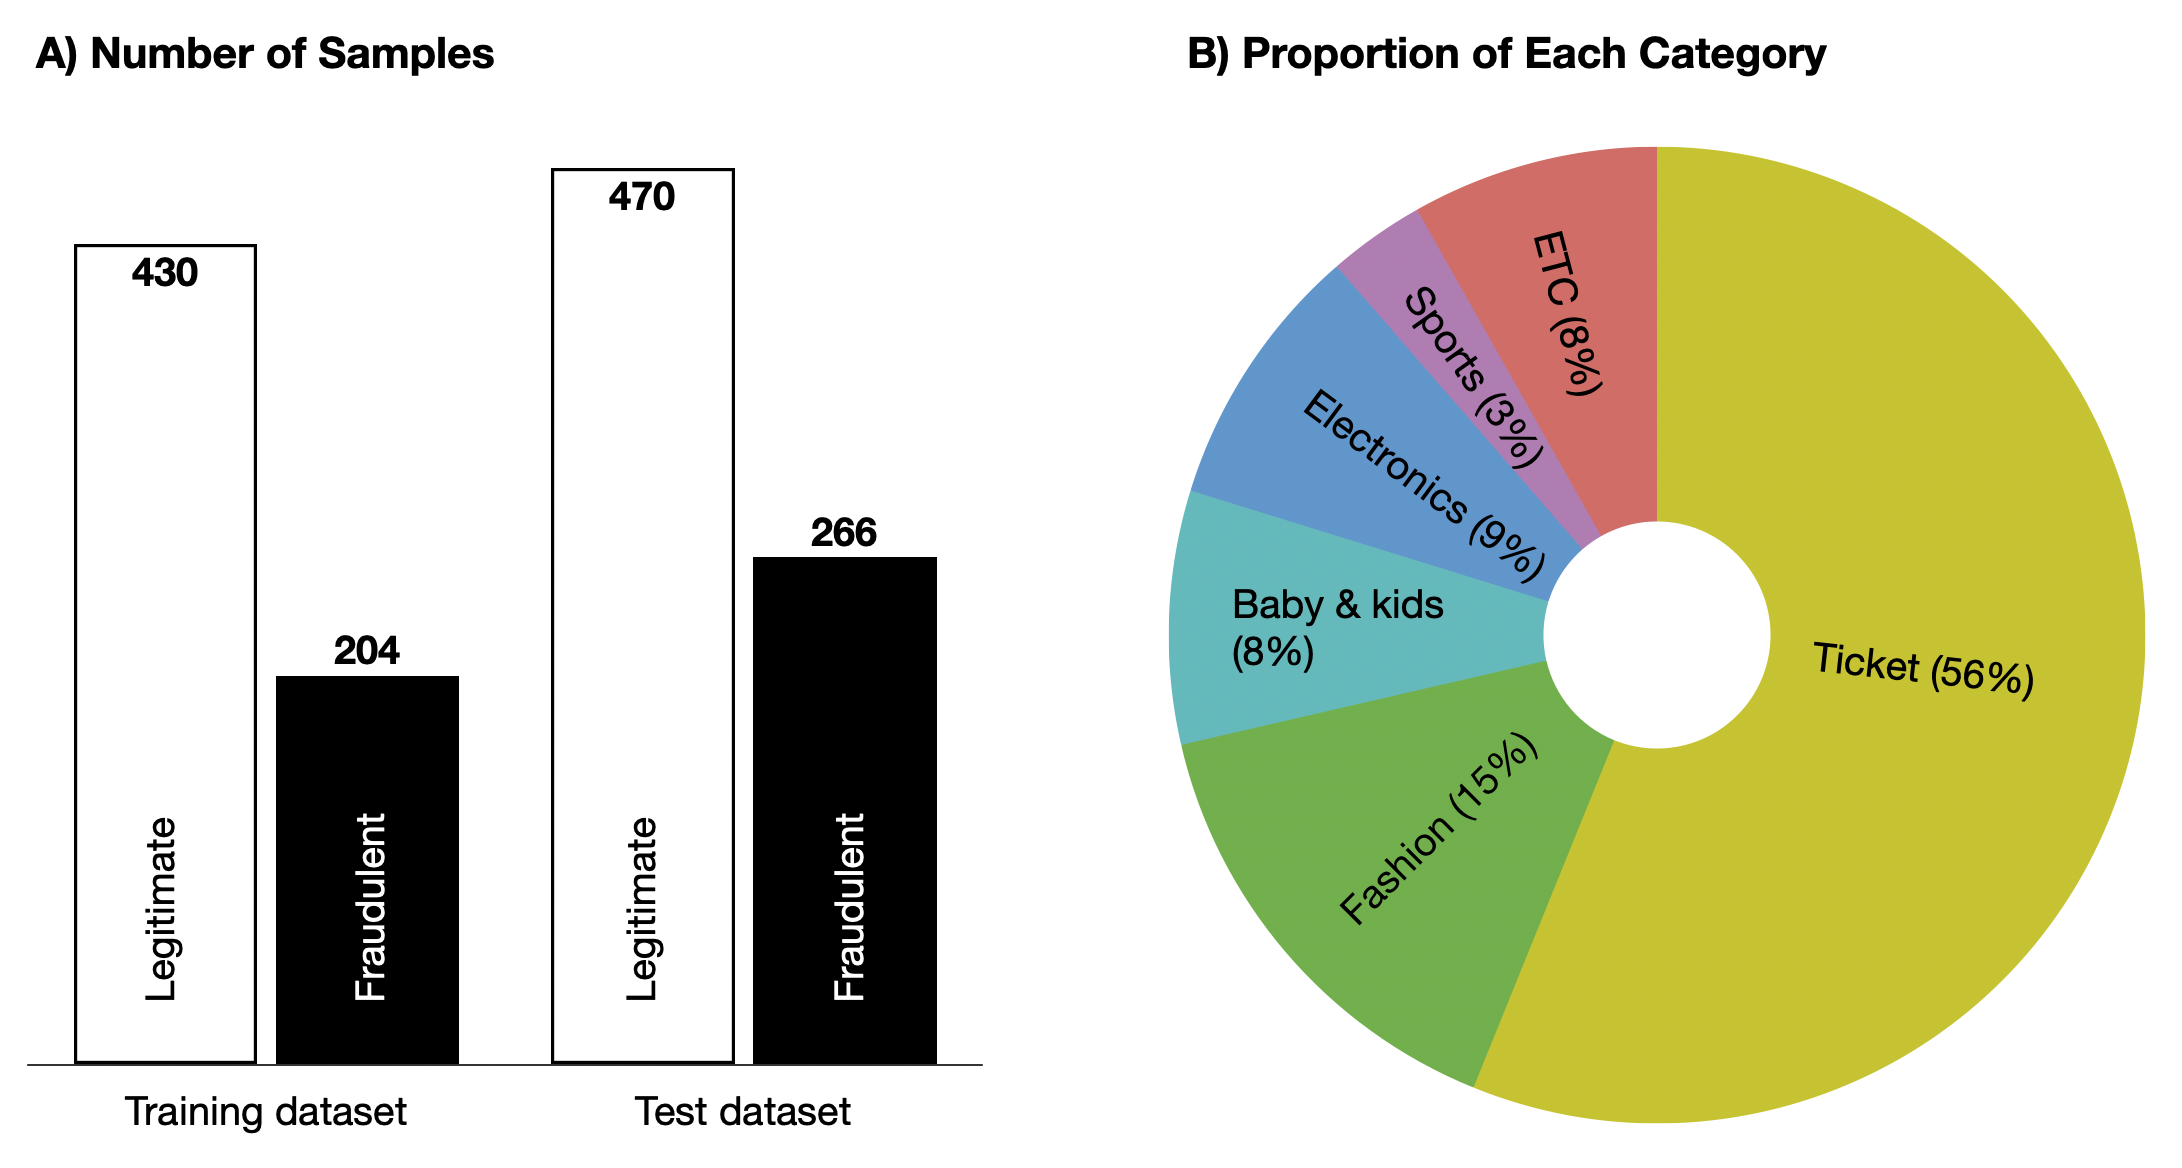
\includegraphics[width=0.48\textwidth]{figures/fig_dataset.png}
  \caption{Overview of the sampled dataset with fraud label distribution}
  \label{fig_dataset}
\end{figure}

\subsection{Category-Wise Distribution}
The sampled transactions span seven major product categories, each exhibiting distinct fraud risk profiles. Table~\ref{tab_category_distribution} summarizes the distribution of fraudulent and legitimate transactions across these categories.


Notably, categories with high liquidity and resale value—such as tickets—exhibit a disproportionately high rate of fraudulent activity. This heterogeneity underscores the importance of incorporating category-specific behavioral patterns into fraud detection models.

\subsection{Feature Overview}
Each transaction instance in the dataset is represented by a set of features grouped into four key dimensions:

\begin{itemize}
    \item \textbf{Listing Metadata}: Includes the listing title (\texttt{title}), asking price (\texttt{price}), and product category (\texttt{category}).
    \item \textbf{Transaction Details}: Captures transaction timestamp (\texttt{tx\_dttm}) and transaction amount (\texttt{tx\_amt}).
    \item \textbf{Seller Profile}: Includes demographic and account-level attributes such as seller age (\texttt{seller\_age}) and account tenure in days (\texttt{seller\_account\_tenure}).
    \item \textbf{Recent Seller Activity}: Summarizes behavioral signals over a 24-hour window preceding the listing. This includes the number of prior transactions (\texttt{recent\_tx\_cnt}), cumulative transaction amount (\texttt{recent\_tx\_amt\_sum}), and number of unique counterparties (\texttt{recent\_unique\_buyers}).
\end{itemize}

These feature groups collectively capture both static attributes and dynamic behavioral cues, facilitating a comprehensive analysis of user behavior for fraud detection.



\begin{table}[b!]
  \centering
  \begin{tabular*}{\columnwidth}{l@{\extracolsep{\fill}}cc}
  \hline
  \textbf{Category} & \textbf{Fraud} & \textbf{Normal} \\
  \hline
  Tickets & 305 & 464 \\
  Fashion \& Miscellaneous & 25 & 184 \\
  Baby \& Kids & 78 & 37 \\
  Electronics & 37 & 84 \\
  Sports & 12 & 32 \\
  Others & 13 & 99 \\
  \hline
  \end{tabular*}
  \caption{Category-wise distribution of the dataset by fraud label}
  \label{tab_category_distribution}
\end{table}


\begin{figure*}[t!]
  \centering
  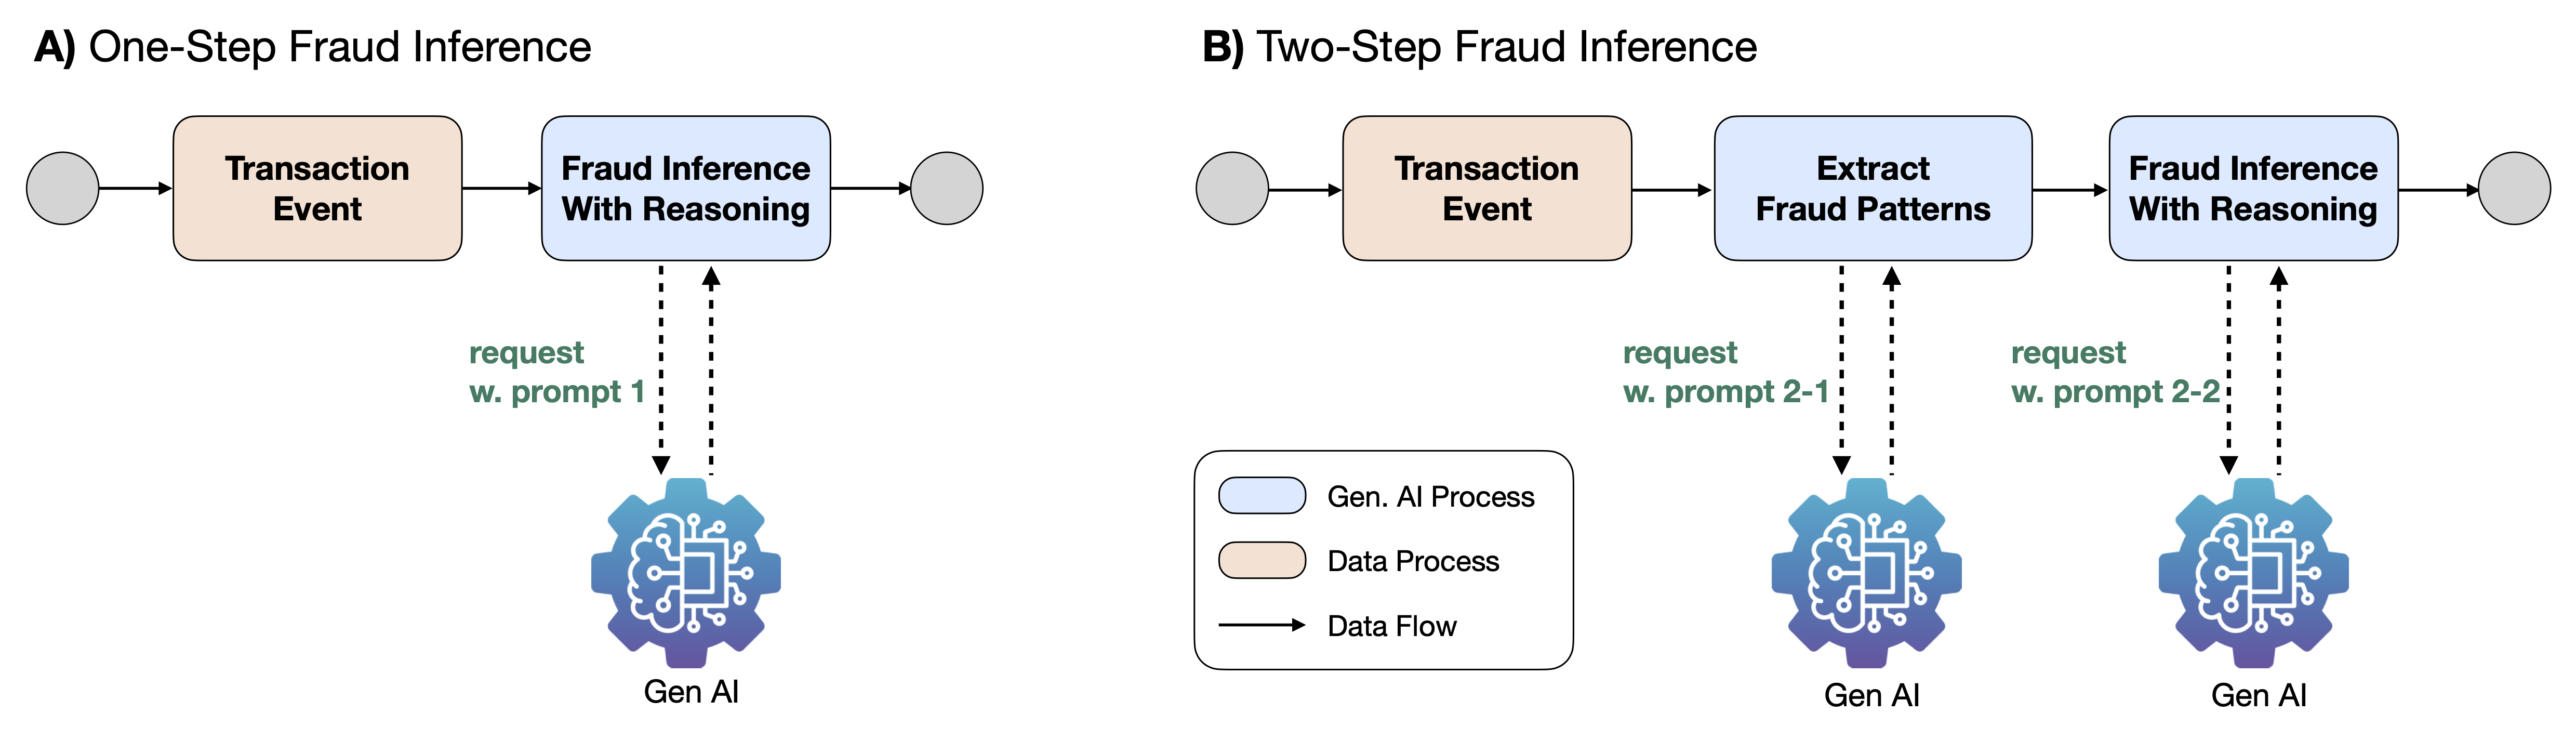
\includegraphics[width=0.9\textwidth]{figures/fig_process.png}
  \caption{Overview of the proposed framework.}
\label{fig_process}
\end{figure*}




% \begin{figure}[t!]
%   \centering
%   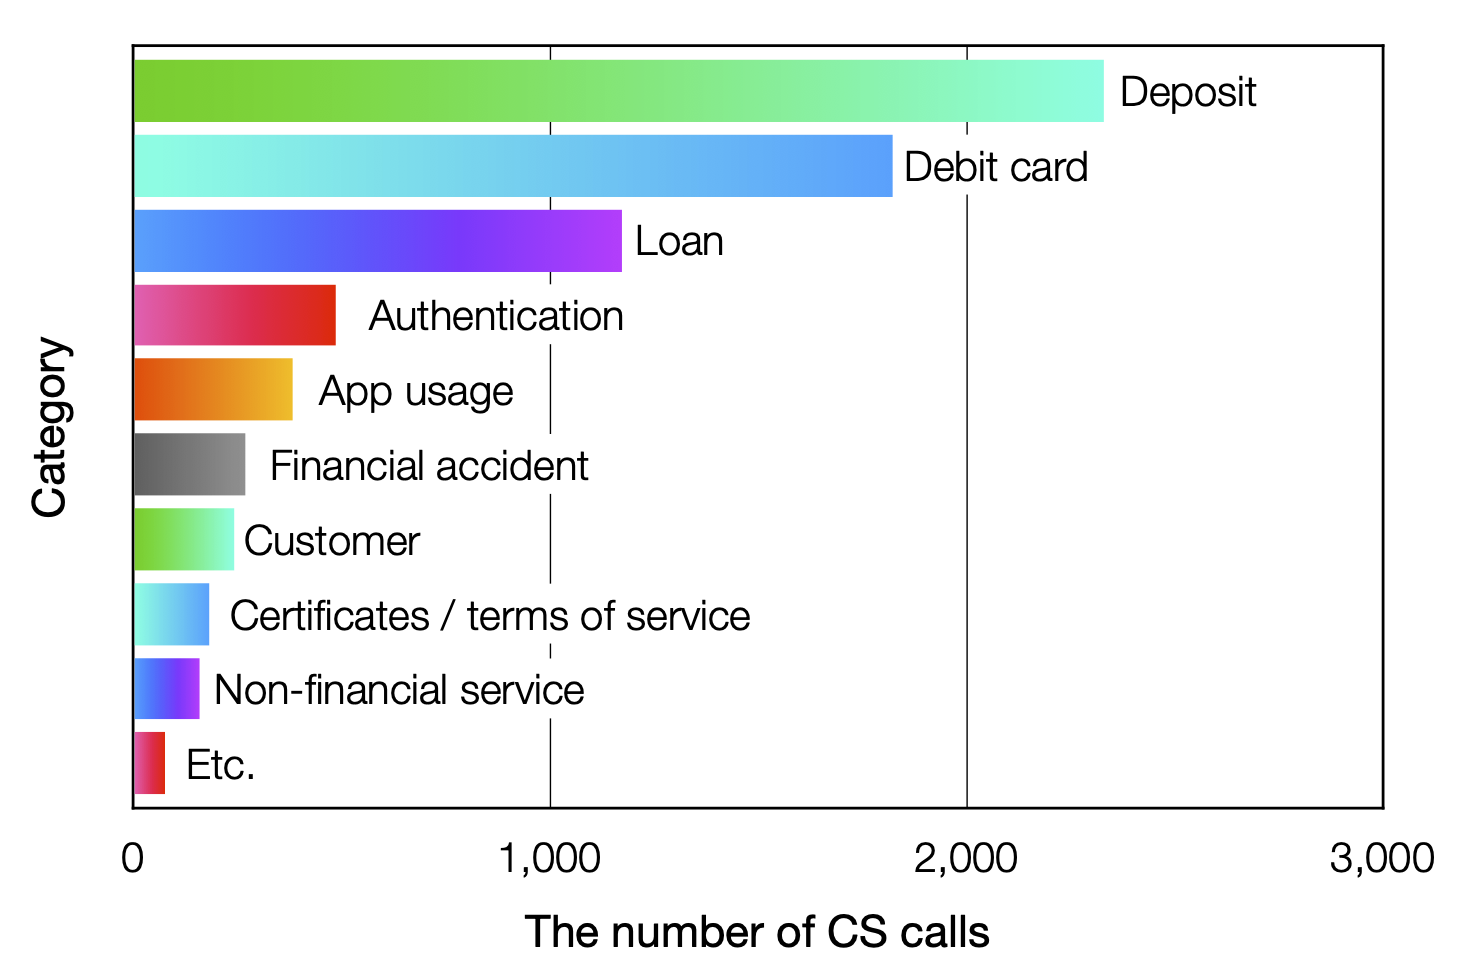
\includegraphics[width=0.48\textwidth]{./figures/fig_cs_category.png}
%   \caption{Number of CS calls in each CS category. 
%   }
% \label{fig_cs_category}
% \end{figure}








\section{Experimental Results}\label{results}
this part is not ready yet.





\subsection{Performance of fine-tuning models}
this part is not ready yet.




% \begin{figure}[t!]
%   \centering
%   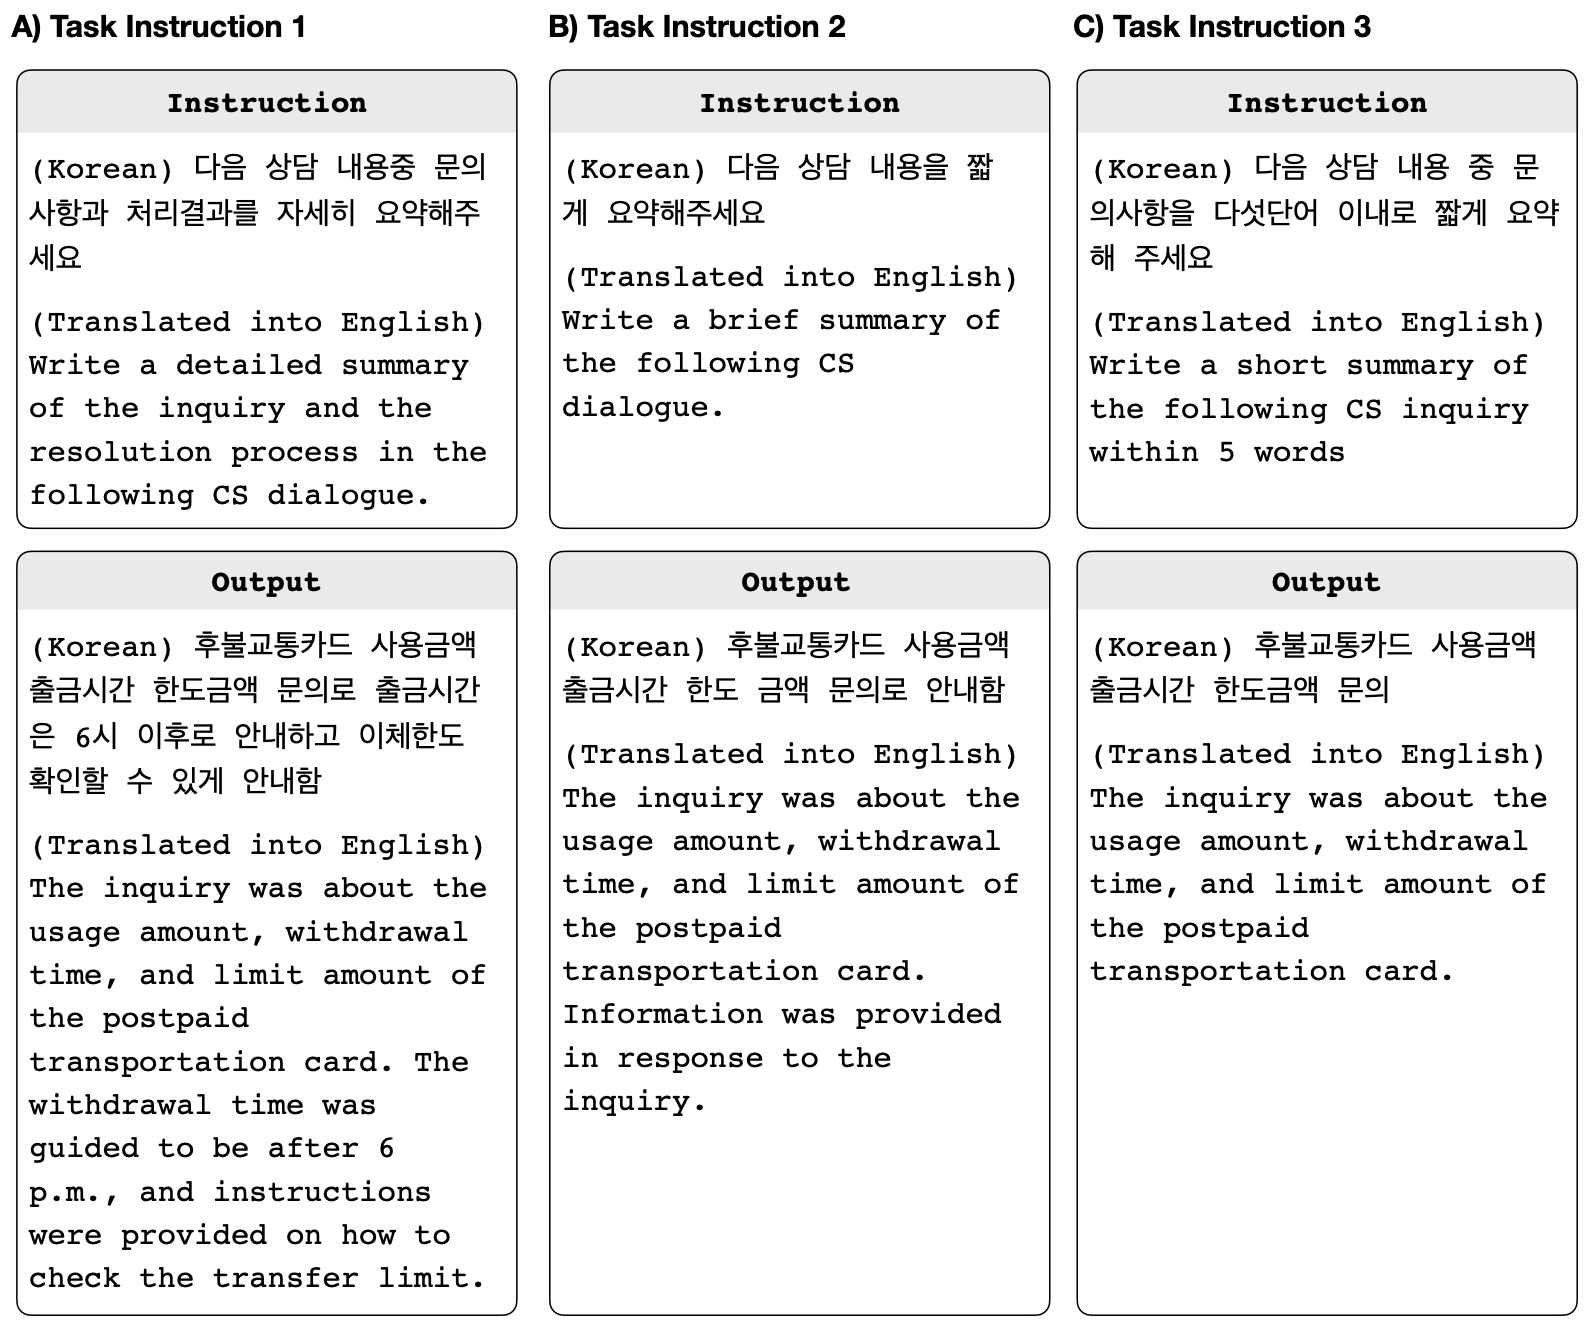
\includegraphics[width=0.48\textwidth]{./figures/fig_var_tasks.png}
%   \caption{Illustrative inference outcomes of the fine-tuning model using multiple instruction templates. The task instructions and their corresponding outputs are demonstrated for (A) an instance of instruction 1 (Write a detailed summary of the inquiry and the resolution process in the following CS dialogue), (B) instruction 2 (Write a brief summary of the following CS dialogue), and (C) instruction 3 (Write a short summary of the following CS inquiry within 5 words). 
%   }
% \label{fig_var_tasks}
% \end{figure}





\section{Conclusions}\label{conclusions}
this part is not ready yet.



%% Print the bibliography
% \printbibliography

\bibliography{references.bib} 



\end{document}
\endinput
%%
%% End of file `sample-sigconf.tex'.
